\section{Question}
A hot tub is 2 m x 2 m square and 1 m tall, and insulated on all sides with polyurethane
foam of thickness 15 cm. Due to mixing issues, the thermistor that measures the water
temperature responds to changes in the average temperature, T, with a time delay of 3
minutes. The hot tub is heated with a resistive heater. \textbf{Design a controller that will
respond to changes in the set point Tsp as fast as possible while being robust to
disturbances. Describe how the controller will be implemented (i.e. what hardware)
and estimate parameters for the controller to the best of your ability.} State any
assumptions.

\subsection *{Answer}

This documents the output of the 90 mins. My hand notes can be found \href{https://bit.ly/test_treau}{here}.

\begin{figure}[h!]
  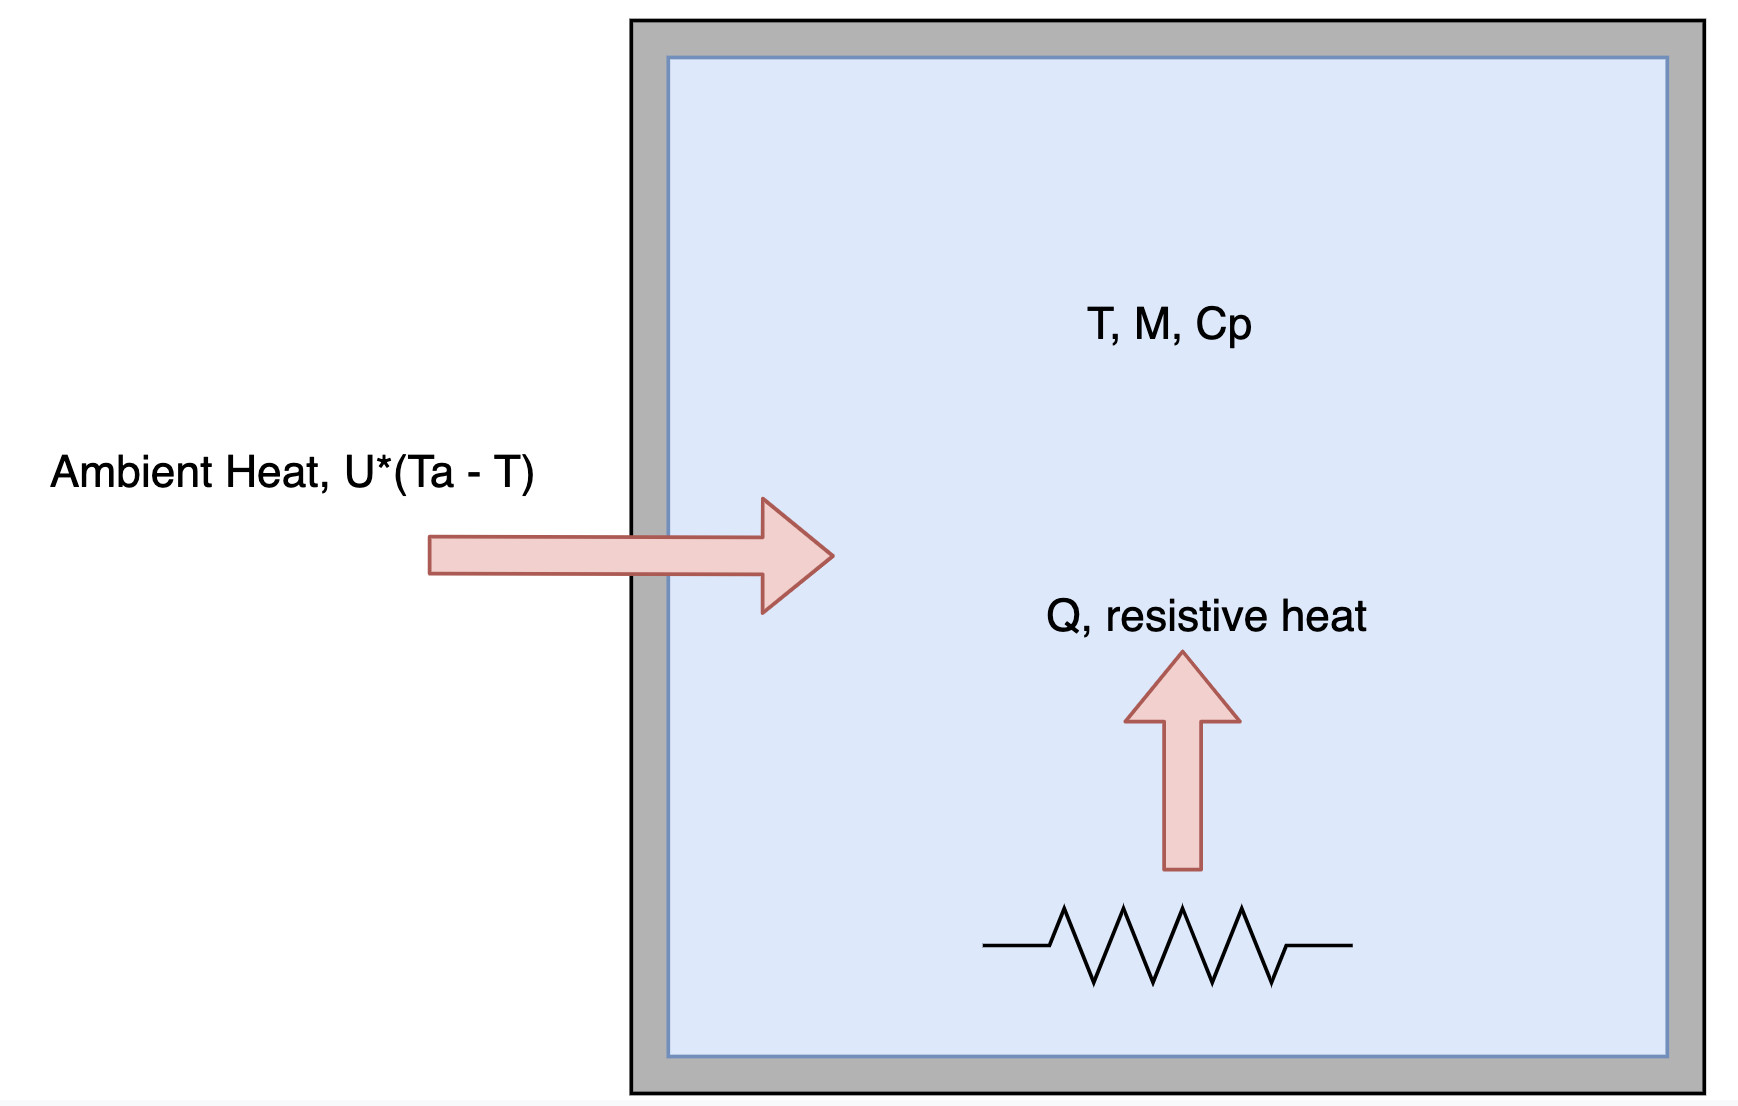
\includegraphics[scale=0.4]{plant}
  \caption{Plant}
\end{figure}

\subsubsection *{Modeling the System}

Thought process:
\begin{enumerate}
  \item The water forms one thermal inertia.
  \item Does the insulation have large enough an inertia to consider it as a second inertia or can I consider this as a purely conductive element? To ascertain this, I calculated the inertia of water and of the polyurethane \href{https://bit.ly/treaucalcs}{here} and found out a ratio of 30:1. So I modeled the polyurethane purely as a conductive element. 
\end{enumerate}

Math Model:
\\
\begin{equation}
\dot{T} = \frac{Q+U*(T_a-T)}{M*C_p}
\end{equation}
where: \\
T - Temperature of hot water tank \\
Q - controlled heat source \\
\(T_a\) - ambient temperature \\
M - mass of water \\
\(C_p\) - specific heat of water \\
\(U = \frac{k*A}{L} \) overall heat transfer coefficient of conduction
\newline
\newline
Rearranging: \\
\begin{equation}
M C_p \dot{T} + U T = Q + U T_a
\end{equation}

\noindent
\newline
This gives a transfer function of temperature over heat input as:
\begin{equation}
G(s) = \frac{T(s)}{Q(s)} = \frac{1}{M C_p s + U}
\end{equation}

%%%%%%%%%%%%%%%%%%%%
\subsection *{Designing the Controller}

Assume that the reference temperature (i.e. desired temperature) is \(T_{ref}\).
\noindent
\newline
\newline
Two considerations for the control design are:
\begin{enumerate}
  \item This is a first order linear system.
  \item This has a time delay.
\end{enumerate}
\noindent
For the first part:
\begin{enumerate}
  \item A feedforward component of \(U*(T_{ref} - T_a)\). I am adding this as there is a delay, so an open loop control will help in reaching the target.
  \item A feedback component \(C(s)\) - proportional control. In reality, a small integrator will also be required as the feedforward will not be perfect. The proportional gain can be tuned using stability/performance criteria.
\end{enumerate}
For the second part, I will augment the controller with a smith predictor. Here is how a smith predictor works:
\begin{enumerate}
  \item The open loop plant dynamics are \(G(s)*e^{-\tau s}\) where \(e^{-\tau s}\) is the laplace transform of the pure delay.
  \item The smith predictor can be understood in two steps:
  \begin{enumerate}
  \item Cancel out \(G(s)*e^{-\tau s}\)
  \item Replace it with the function \(G_p(s)\), which is a simulated version of \(G(s)\)
  \end{enumerate}
  \item The controller can be tuned for \(G(s)\), i.e. the \textit{plant without the delay} with a smith predictor.
\end{enumerate}

\noindent
\newline
The process diagram with the controller is shown below. For reference, \textbf{blocks highlighted in \textcolor{TealBlue}{blue} are in in the ECU}, the rest is the real plant: \\

\begin{figure}[h!]
  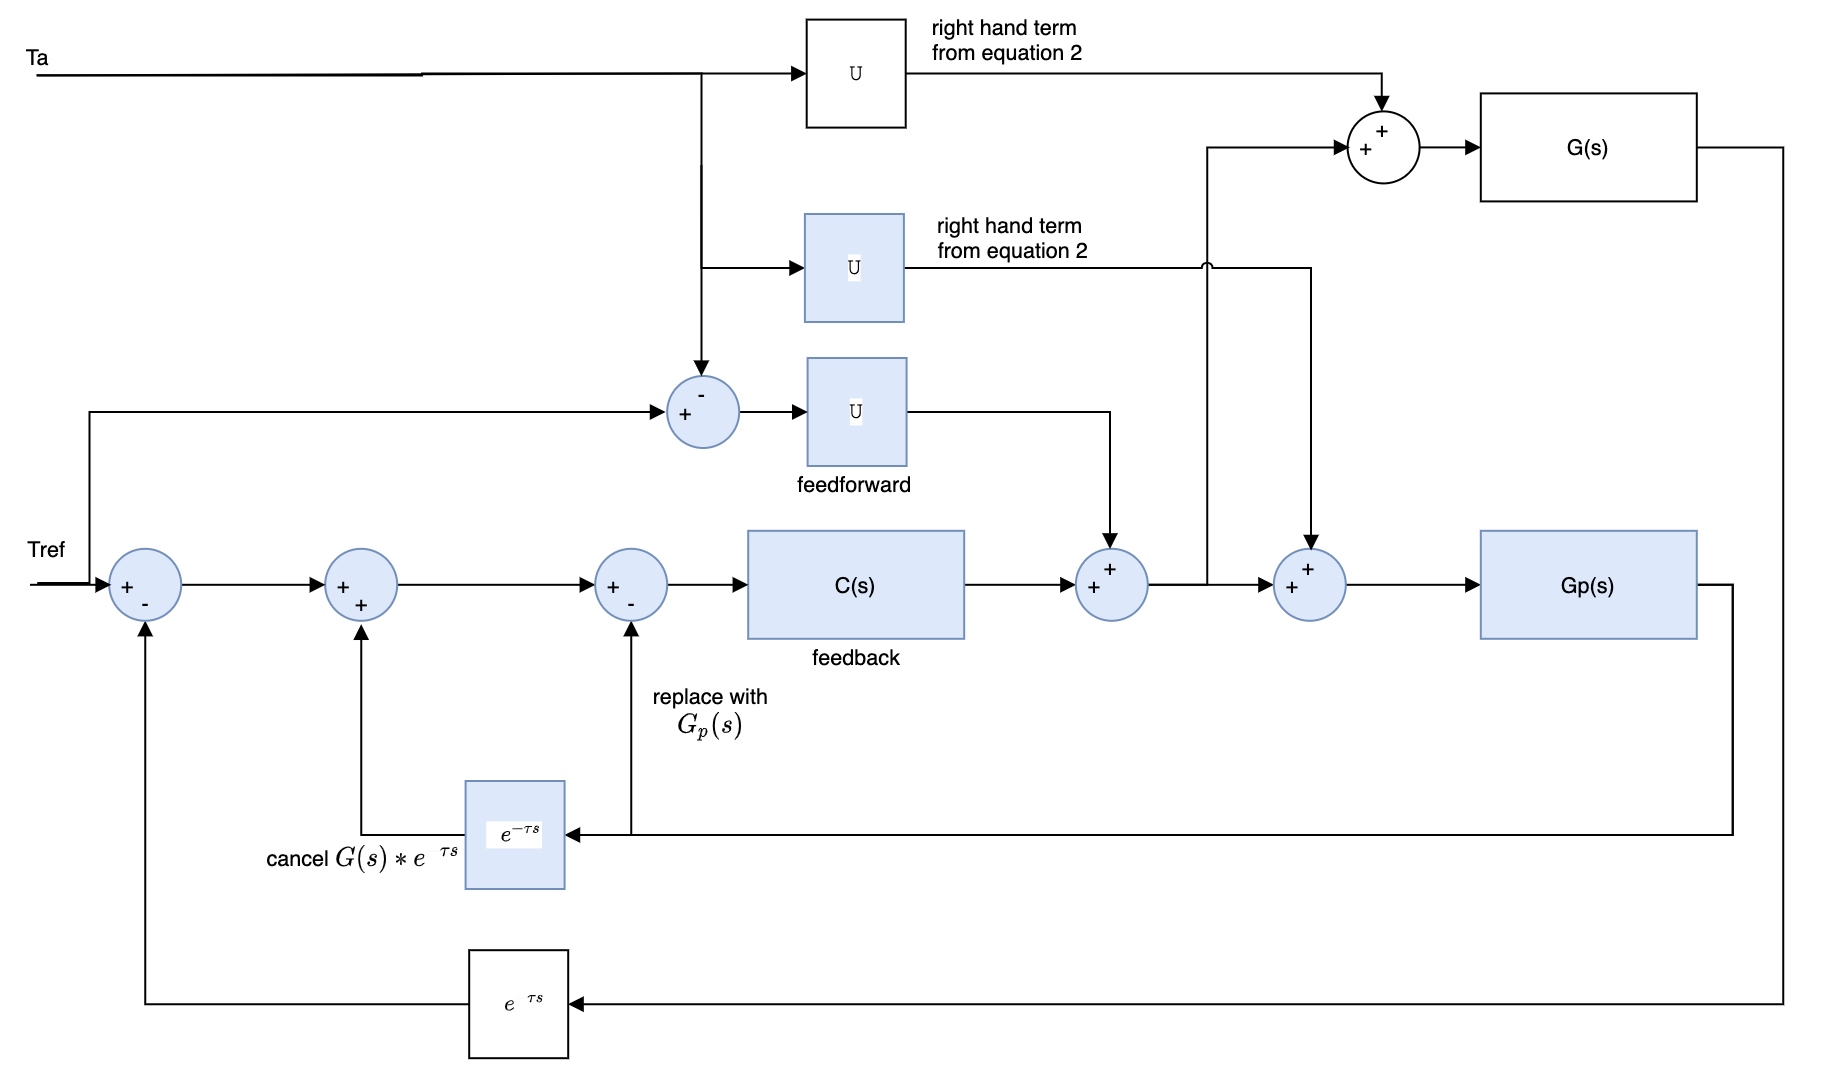
\includegraphics[width=\textwidth]{control_diagram}
  \caption{Process Diagram}
\end{figure}

%%%%%%%%%%%%%%
\subsection *{Parameters}
I used for polyurethane:
cp = 1800 J/kg-K
density = 132.953 Kg/$m^3$
conduction coefficient = 0.03 W/mK
\noindent
The closed loop transfer function with a proportional controller was:
\begin{equation}
G(s) = \frac{T(s)}{Q(s)} = \frac{K}{M C_p s + U + K} = \frac{K}{1.68 *10^7 s + 3.2 + K}
\end{equation}
\noindent
If I introduce a time constant requirement of 200 seconds, I get an extremely high gain of K = 82000. I googled residential hot water tanks and this gain would make the system be out of its actuating range for the most part.

%%%%%%%%%%%%%%
\subsection *{Hardware}
\begin{itemize}
  \item Thermistor - connected to ADC input with appropriately sized voltage divider circuit
  \item Resistive heater - not sure how this is throttled. If this was running off DC, I would use a half bridge that would have a PWM signal going to it from the micro.
  \item A micro of course for running the software.
  \item To input set temperature. Potentiometer to an ADC input.
  \item Display for temperature.
\end{itemize}